%!TEX root = main.tex

\section{Kapitel 3: Pointer und Referenzen\hfill}
\label{sec:abschnitt}

\subsection{Höhere und strukturierte Datentypen\hfill}
\label{sec:unterabschnitt}

\subsubsection{Höhere Datentypen\hfill}
\label{sec:unterunterabschnitt}
\begin{itemize}
	\item Pointer
	\item Referenzen
	\item Vektoren
\end{itemize}

\subsubsection{Strukturierte Datentypen\hfill}
\label{sec:unterunterabschnitt}
\begin{itemize}
	\item Strukturen
	\item Klassen
\end{itemize}

% Unterkapitel: Pointer

\subsection{Pointer\hfill}
\label{sec:unterabschnitt}

\subsubsection{Adresse\hfill}
\label{sec:unterunterabschnitt}
\begin{itemize}
	\item Die Nummereiner Speicherzelle wird als \textbf{Adresse} bezeichnet
	\item Bei einem byteweise adressierbaren Speicher(ist üblich) liegt an jeder Adresse genau 1 Byte
\end{itemize}

\subsubsection{Pointer\hfill}
\label{sec:unterunterabschnitt}
\begin{itemize}
	\item Synonym: Zeiger
	\item Ein Pointer ist eine Variable, welche die Adresse einer im Speicher befindlichen Variablen oder Funktion aufnehmen kann
	\item Man sagt, der Pointer zeige (to point) auf diese Speicherzelle
	\item Pointer in C++ sind zu 99.99\% identisch zu Pointern in C
\end{itemize}

\subsubsection{Standarddarstellung von Pointern\hfill}
\label{sec:unterunterabschnitt}
\noindent
\begin{minipage}{\linewidth}
\begin{lstlisting}
float alpha;
float* pointer;
alpha = 1.4f;
pointer = \&alpha;
 \end{lstlisting}
\end{minipage}
\begin{figure}[h]
	\centering
	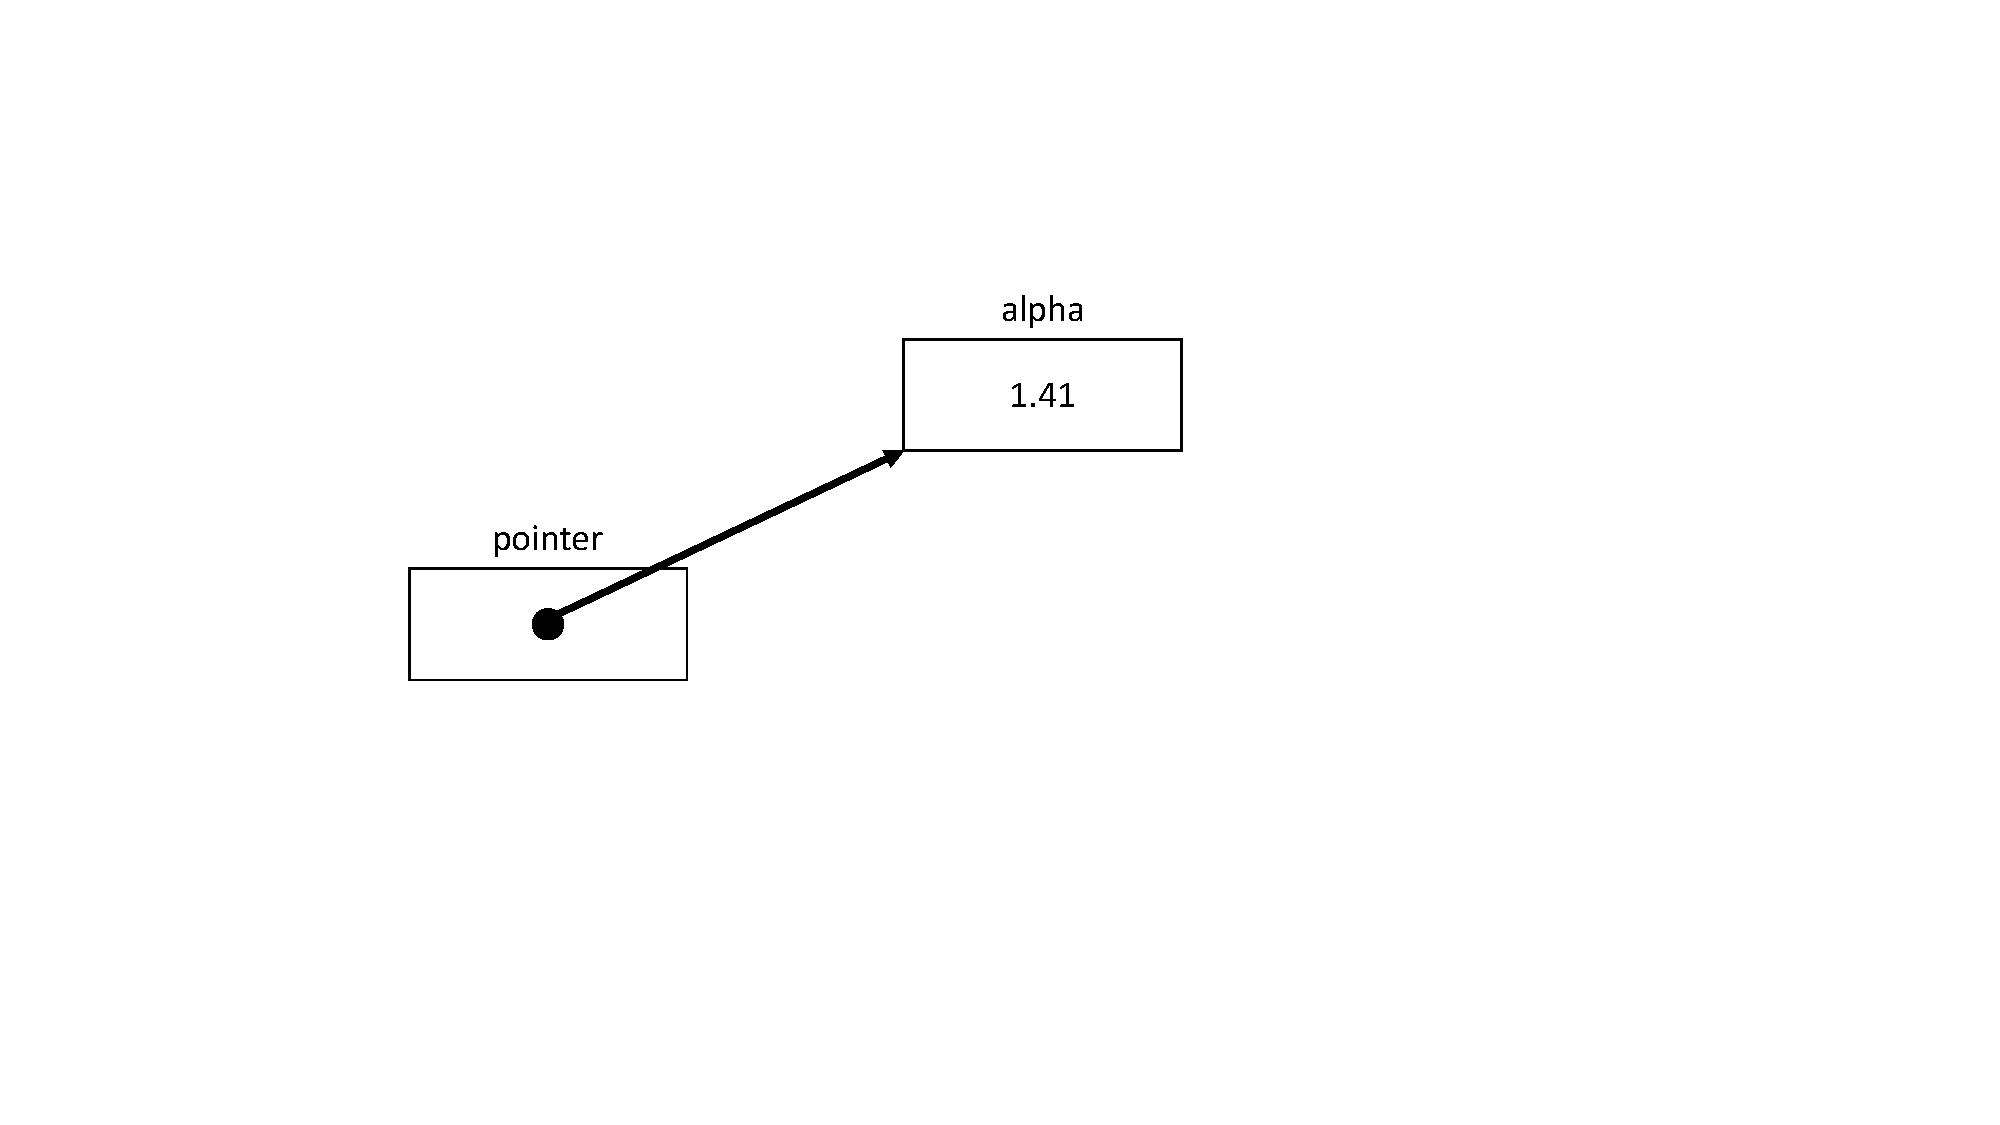
\includegraphics[width=0.4\linewidth]{pointer1.pdf}
\end{figure}

\subsubsection{Pointer und Datentyp\hfill}
\label{sec:unterunterabschnitt}
\begin{itemize}
	\item Pointer in C++ sind typisiert (wie in C), sie zeigen auf eine Variable des definierten Typs
	\item Oder anders ausgedrückt:
		\\ Der Speicherbereich, auf den ein bestimmter Pointer zeigt, wird entsprechend des definierten Pointer-Typs interpretiert
	\item Der Speicherbedarf einer Pointervariablen ist unabhängig vom Pointer-Typ. Er ist so gross, dass die maximale Adresse Platz findet
		\\ (z.B. 32 Bits für $2^{32}$ Adressen)
\end{itemize}

\subsubsection{Definition einer Pointervariablen\hfill}
\label{sec:unterunterabschnitt}
\noindent
\begin{minipage}{\linewidth}
\begin{lstlisting}
*@// Datentyp des Pointers	Kennzeichnung des Pointers durch '\color{blue}*\color{black}'@*
*@\color{red}Typname\color{blue}* \color{black} pointerName;@*

// Konkrete Beispiele:

int* ptr1;		// ptr1 ist ein Pointer auf int
double* ptr2;	// ptr2 ist ein Pointer auf double
\end{lstlisting}
\end{minipage}
\begin{figure}[h]
	\centering
	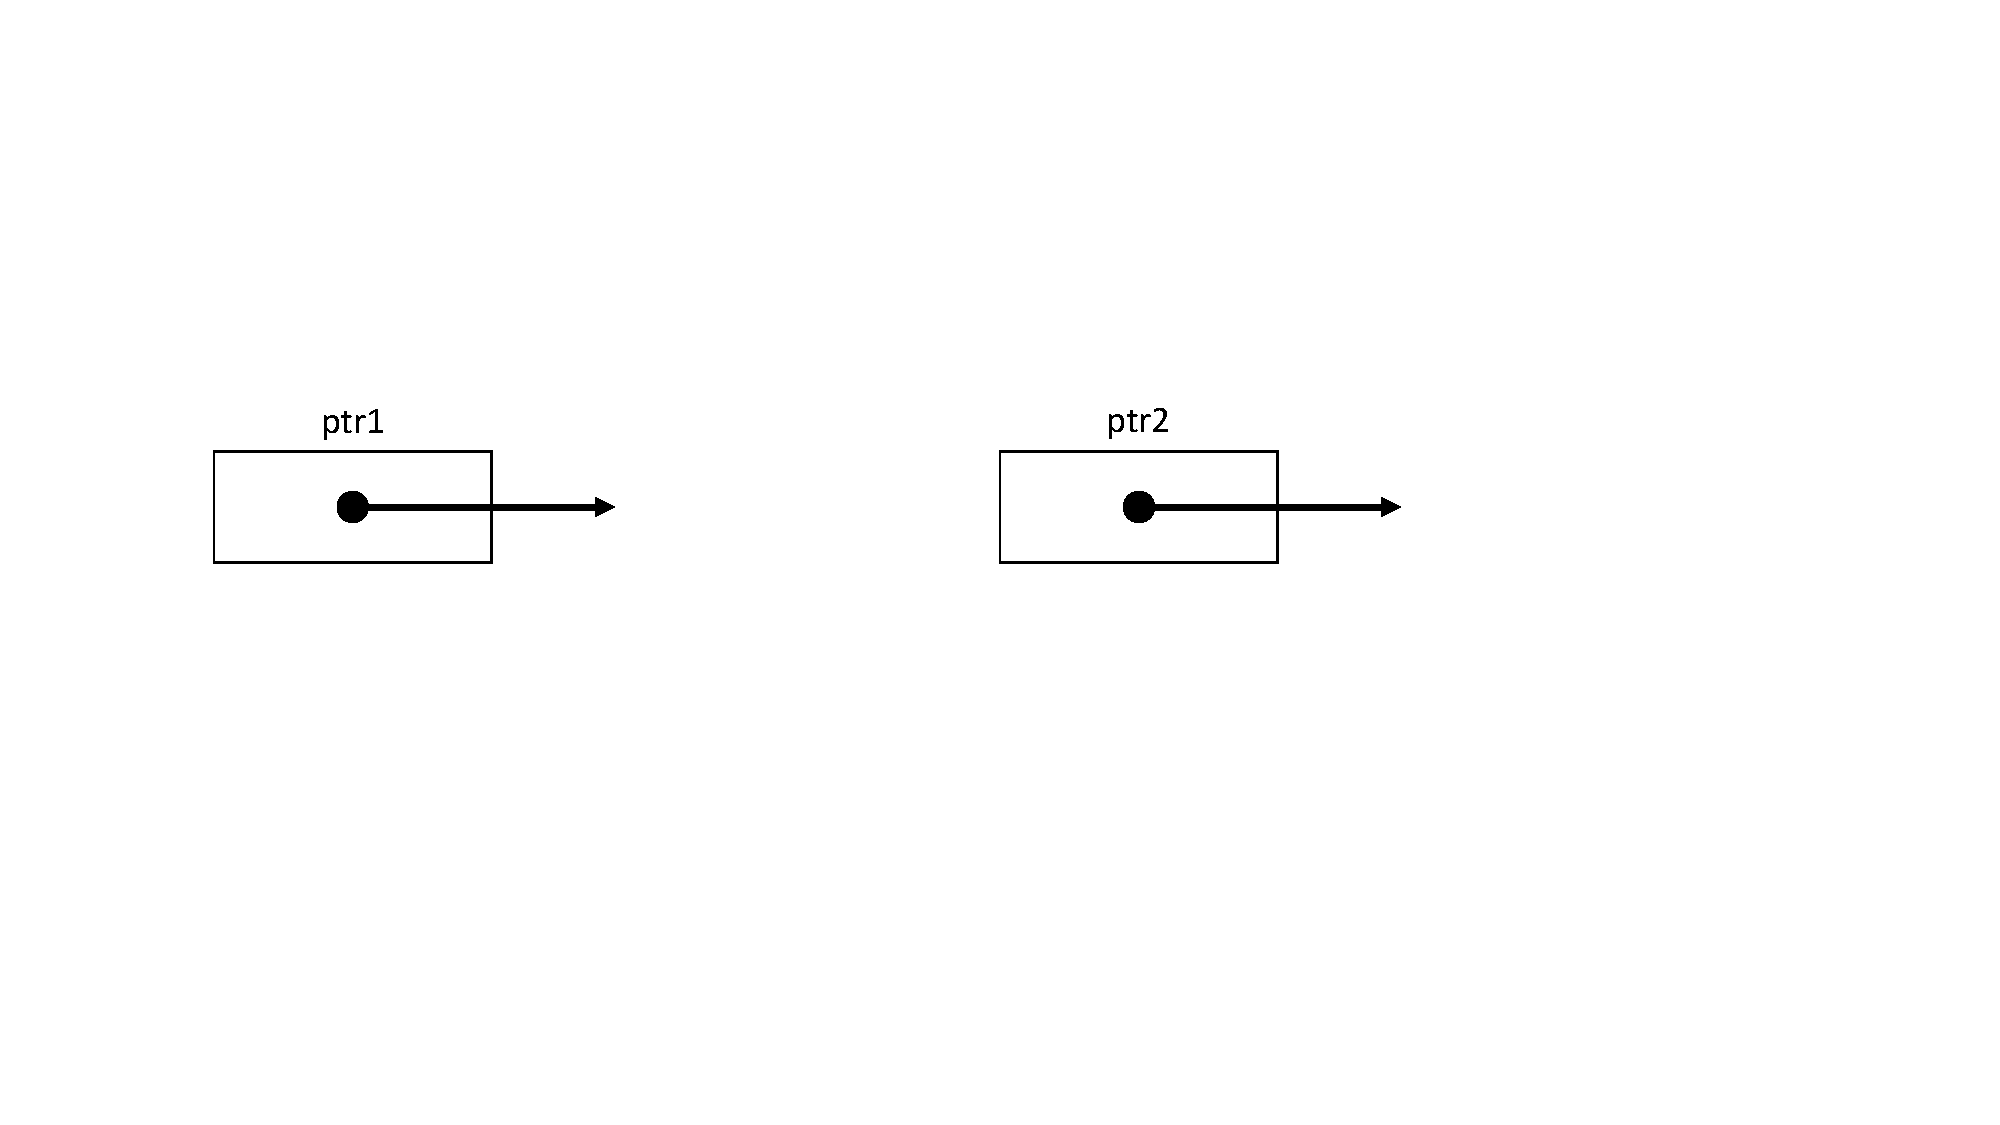
\includegraphics[width=0.5\linewidth]{pointer2.pdf}
\end{figure}

\subsubsection{Initialisierung mit Null-Pointer\hfill}
\label{sec_unterunterabschnitt}
Mit dem Null-Pointer wird angezeigt, dass der Pointer auf \textbf{kein} Objekt zeigt. Dem Pointer wird ein definierter Nullwert zugewiesen.\\
\\
\begin{hinweis}
Der Pointer zeigt nicht auf die Adresse 0!
\end{hinweis}
\\
\\
\noindent
\begin{minipage}{\linewidth}
\begin{lstlisting}
int* ptr = 0;	// bitte nicht NULL verwenden!
\end{lstlisting}
\end{minipage}
\begin{figure}[h]
	\centering
	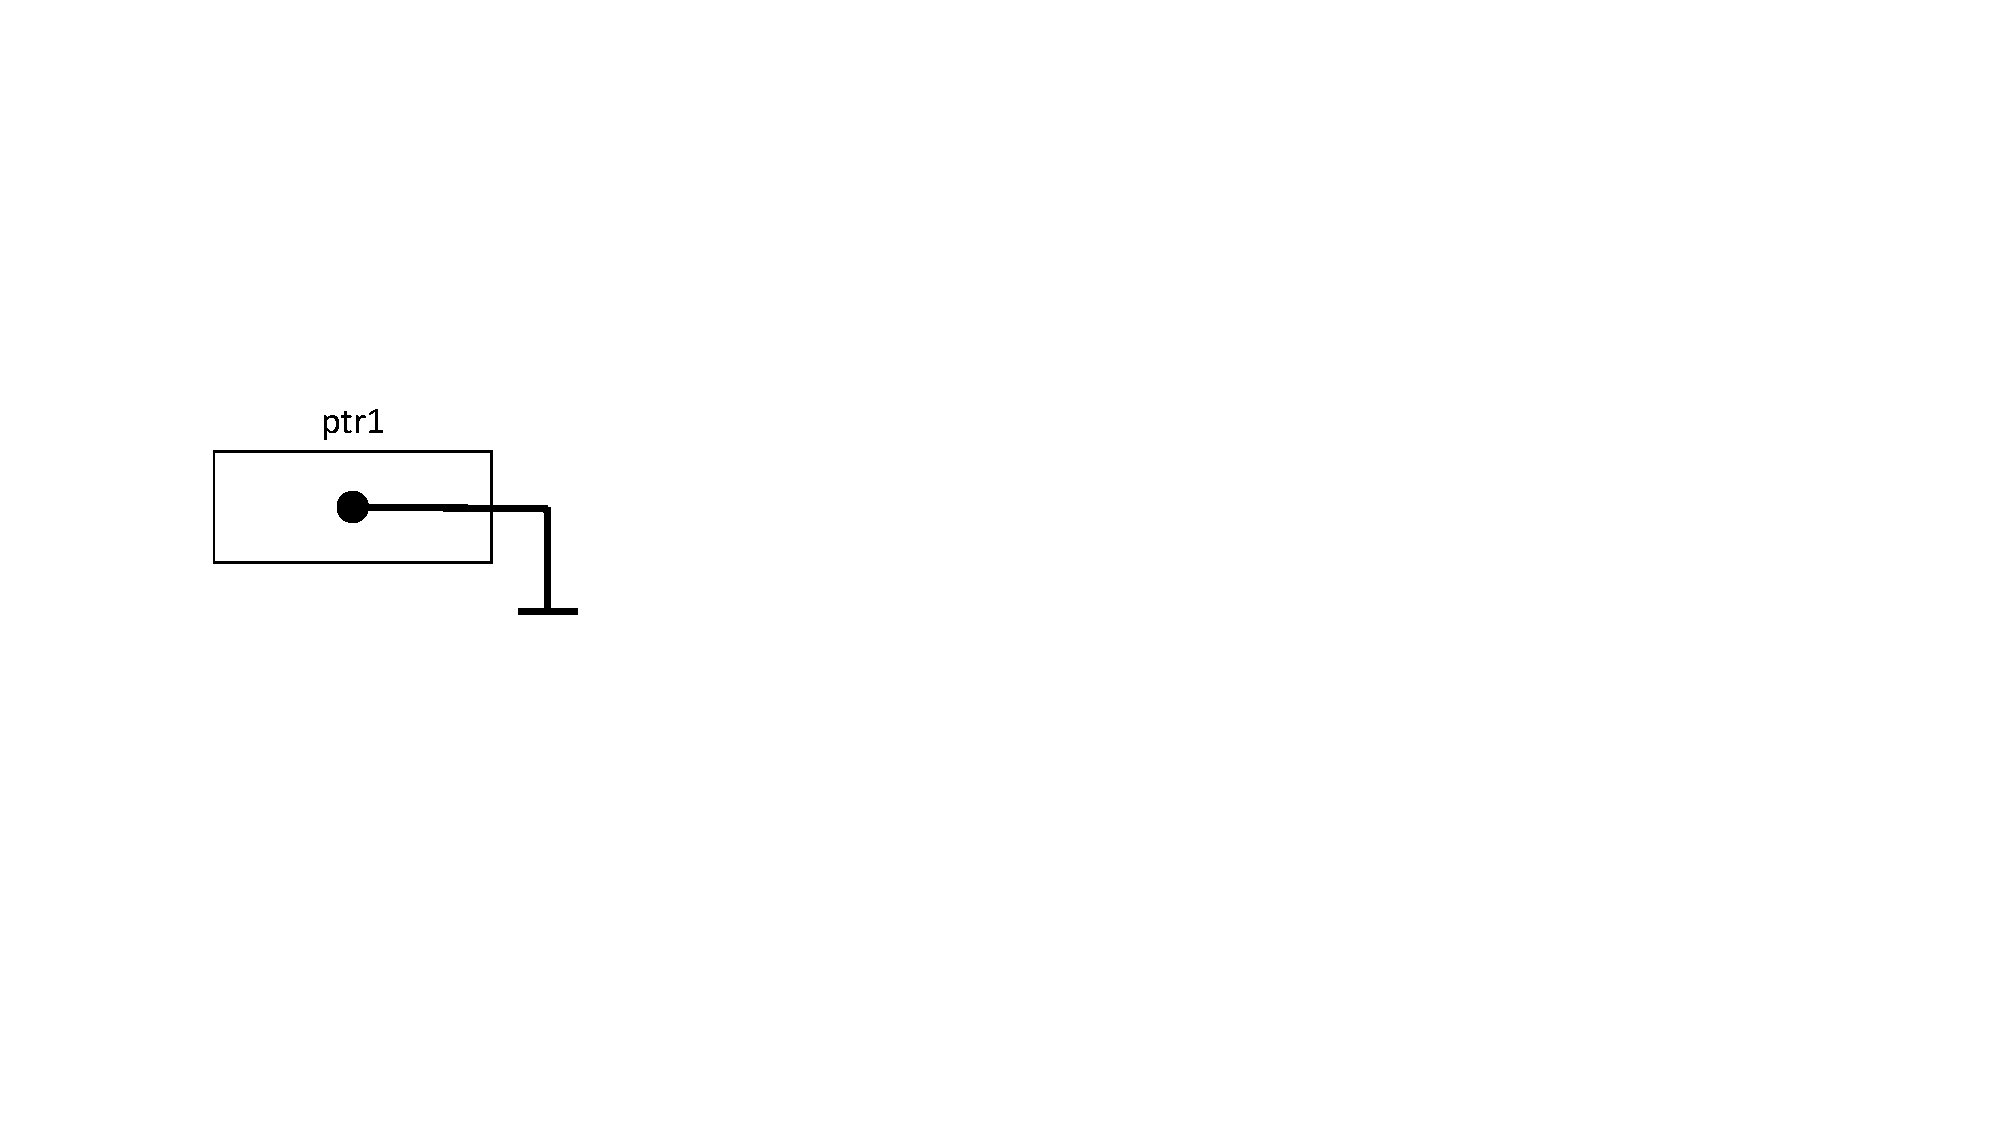
\includegraphics[width=0.2\linewidth]{pointer3.pdf}
\end{figure}

\subsubsection{Der Adressoperator \& \textbf{(Referenzierung)}\hfill}
\label{sec:unterunterabschnitt}
Ist x eine Variable vom Typ Typname, so liefert der Ausdruck \&x einen Pointer auf die Variable x, d.h. er liefert die Adresse der Variablen x.\\
\\
\noindent
\begin{minipage}{\linewidth}
\begin{lstlisting}
int wert;		// Variable wert vom Typ int wird definiert
int* ptr;		// Pointer ptr auf den Typ int wird definiert
			// ptr zeigt auf eine nicht definierte Adresse
		
ptr = &wert;		// ptr zeigt nun auf die Variable wert, d.h. 
			// ptr enthaelt die Adresse der Variablen wert
\end{lstlisting}
\end{minipage}

\subsubsection{Kopieren von Adressen\hfill}
\label{sec:unterunterabschnitt}
\noindent
\begin{minipage}{\linewidth}
\begin{lstlisting}
float alpha;
float* ptr1 = &alpha;
\end{lstlisting}
\end{minipage}
\begin{figure}[h!]
	\centering
	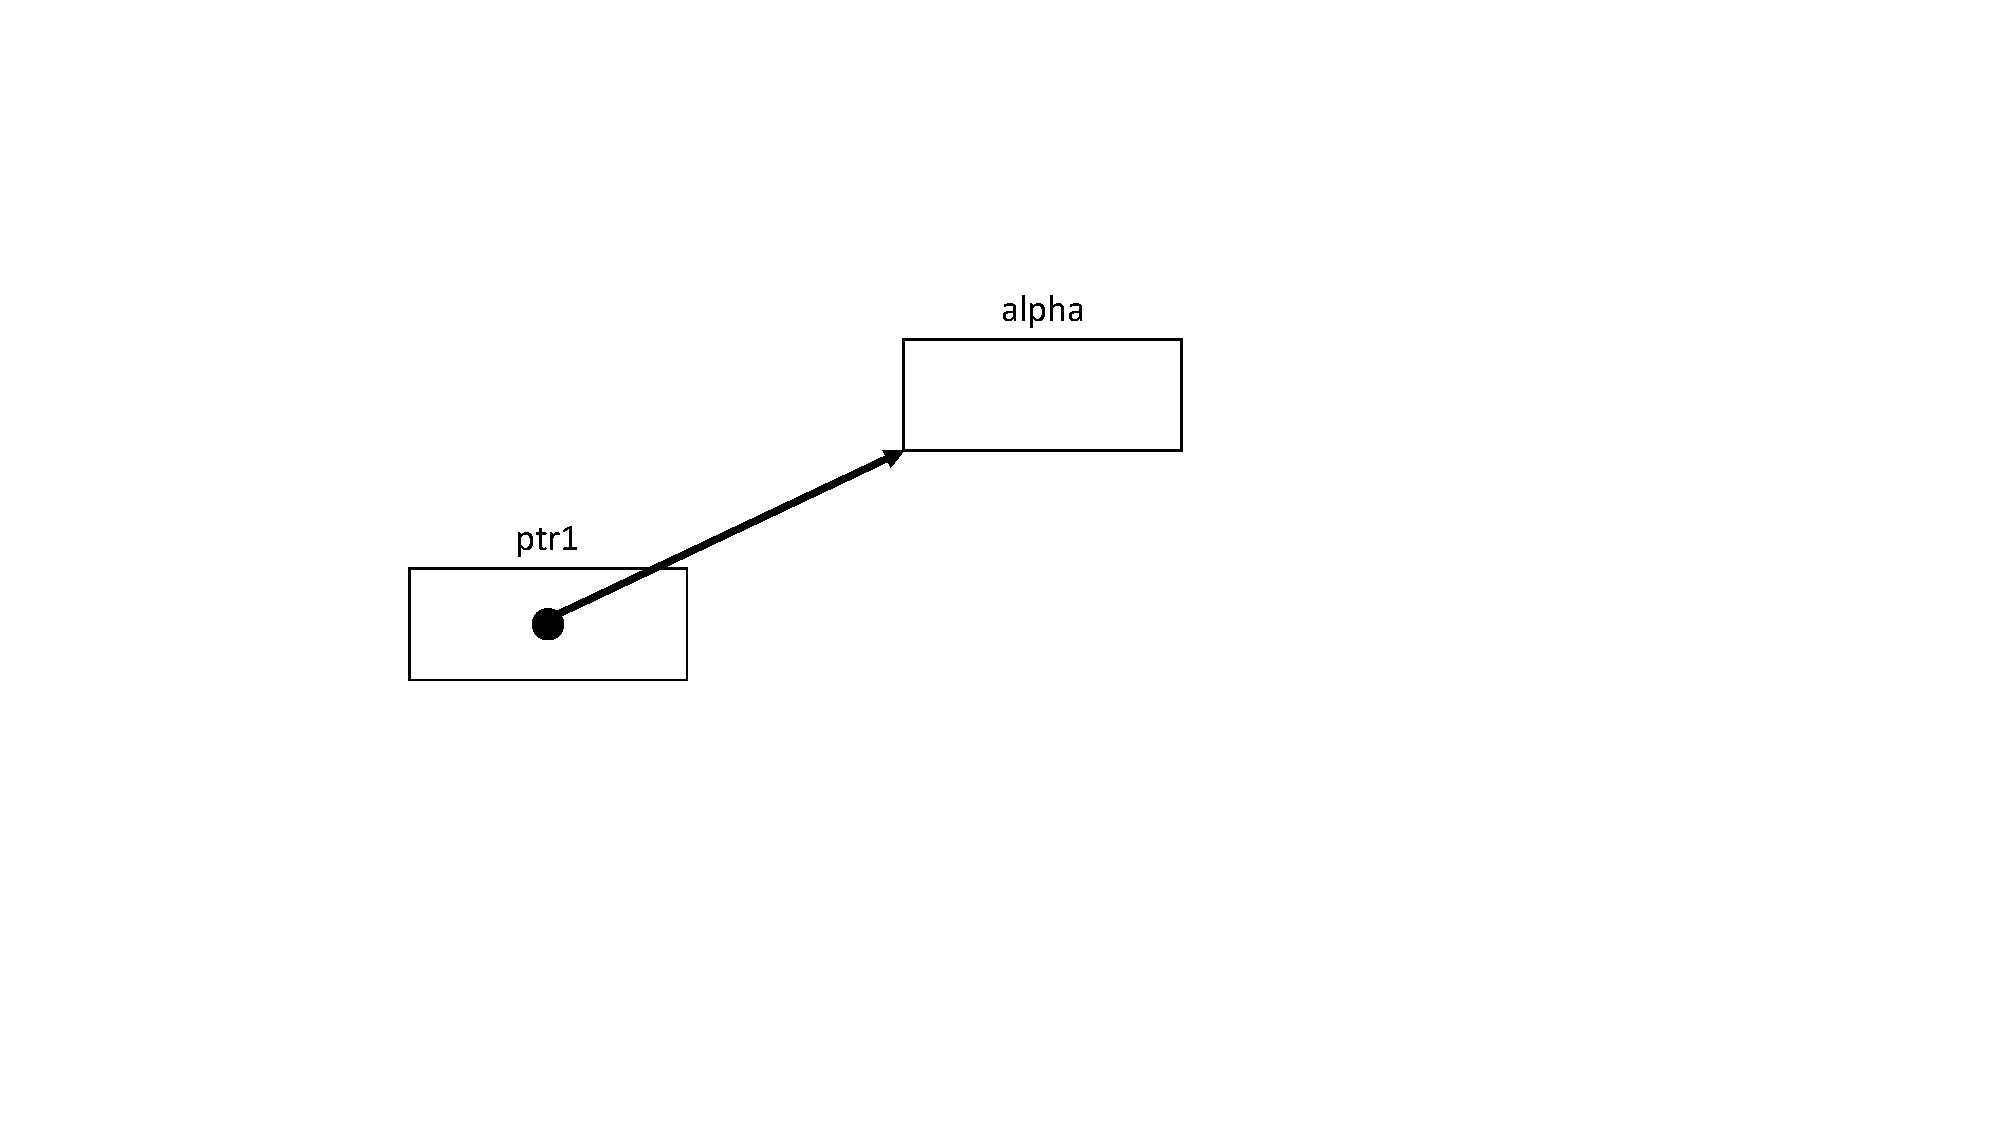
\includegraphics[width=0.4\linewidth]{pointer4.pdf}
\end{figure}
\\ \\ \\
\noindent
\begin{minipage}{\linewidth}
\begin{lstlisting}
float* ptr2;
\end{lstlisting}
\end{minipage}
\begin{figure}[h!]
	\centering
	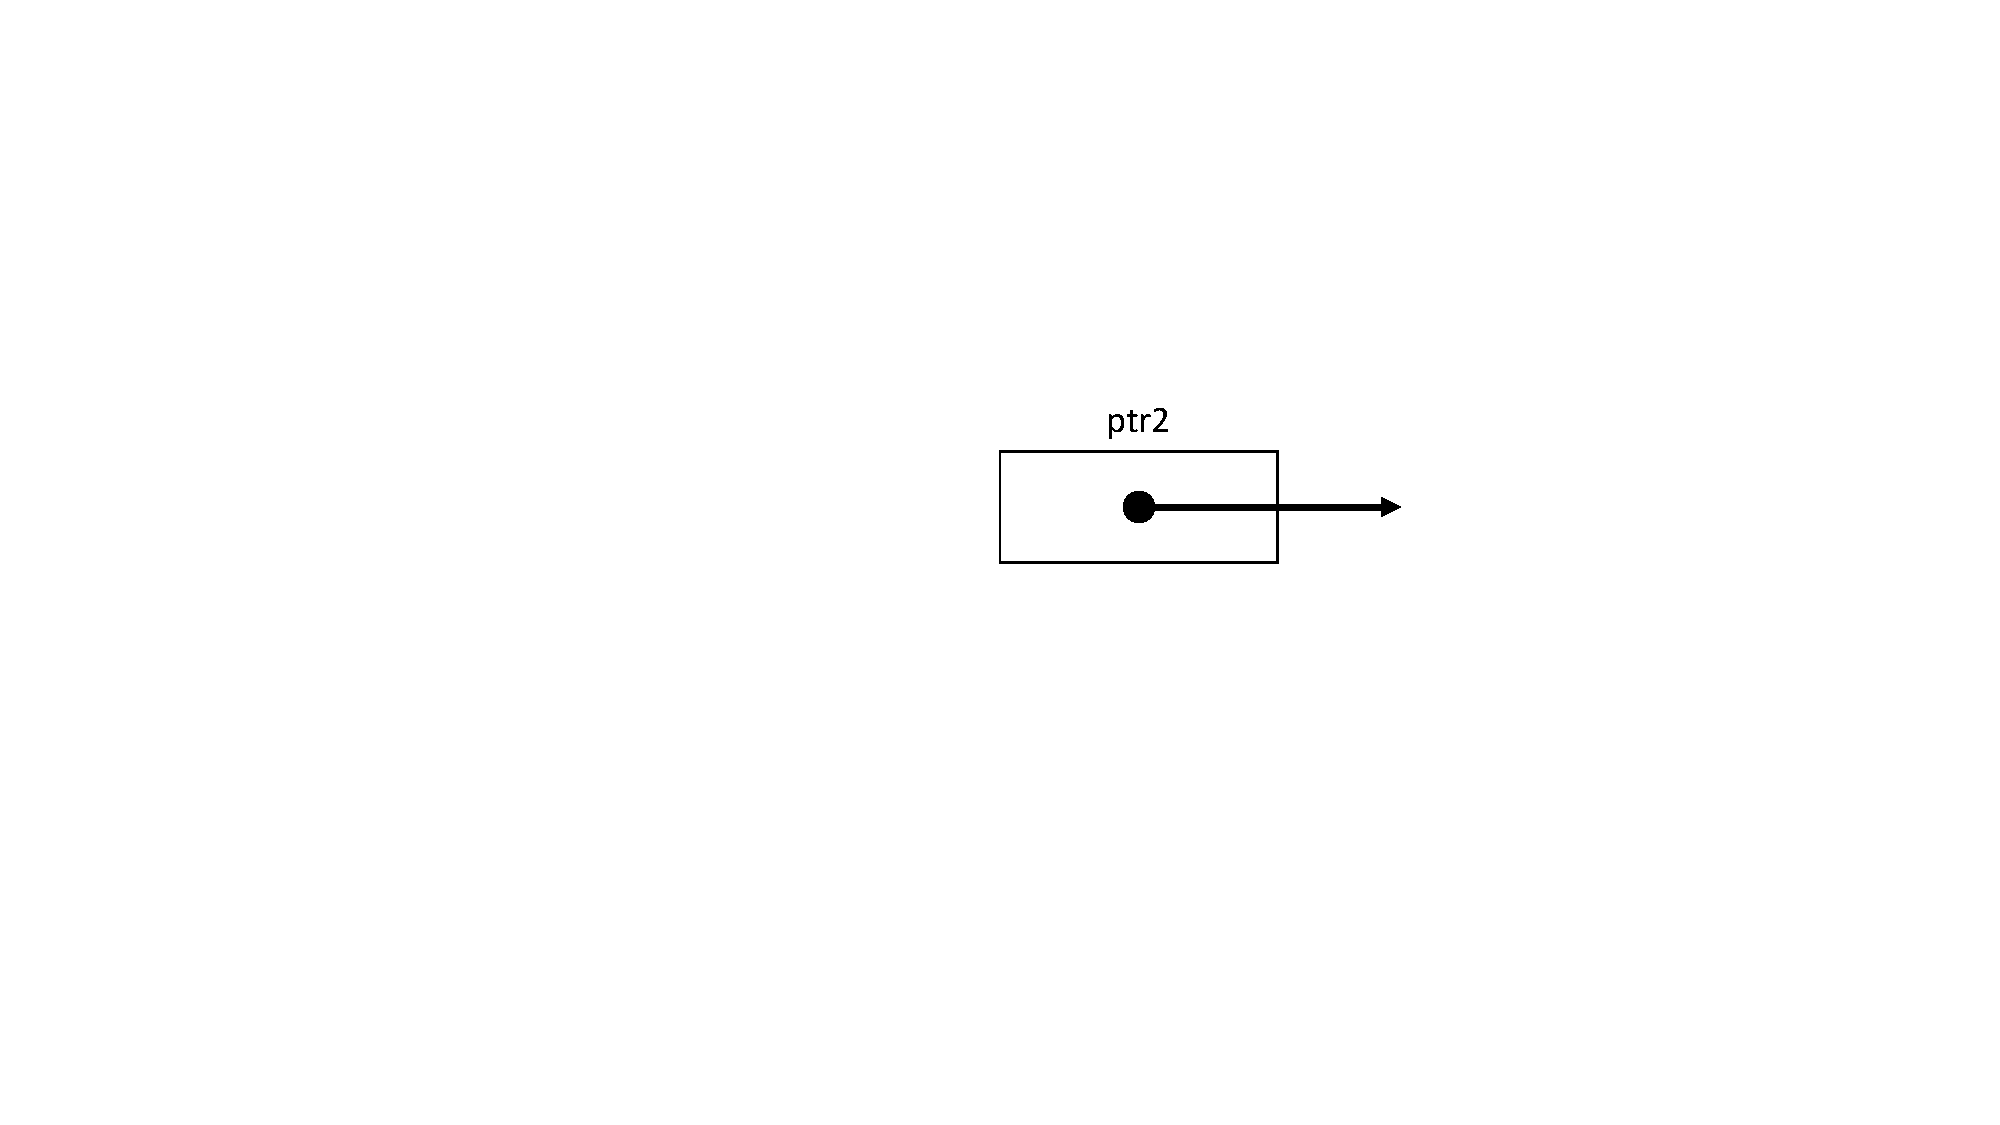
\includegraphics[width=0.2\linewidth]{pointer5.pdf}
\end{figure}
\\ \\ \\
\noindent
\begin{minipage}{\linewidth}
\begin{lstlisting}
ptr2 = ptr1;
\end{lstlisting}
\end{minipage}
\begin{figure}[h!]
	\centering
	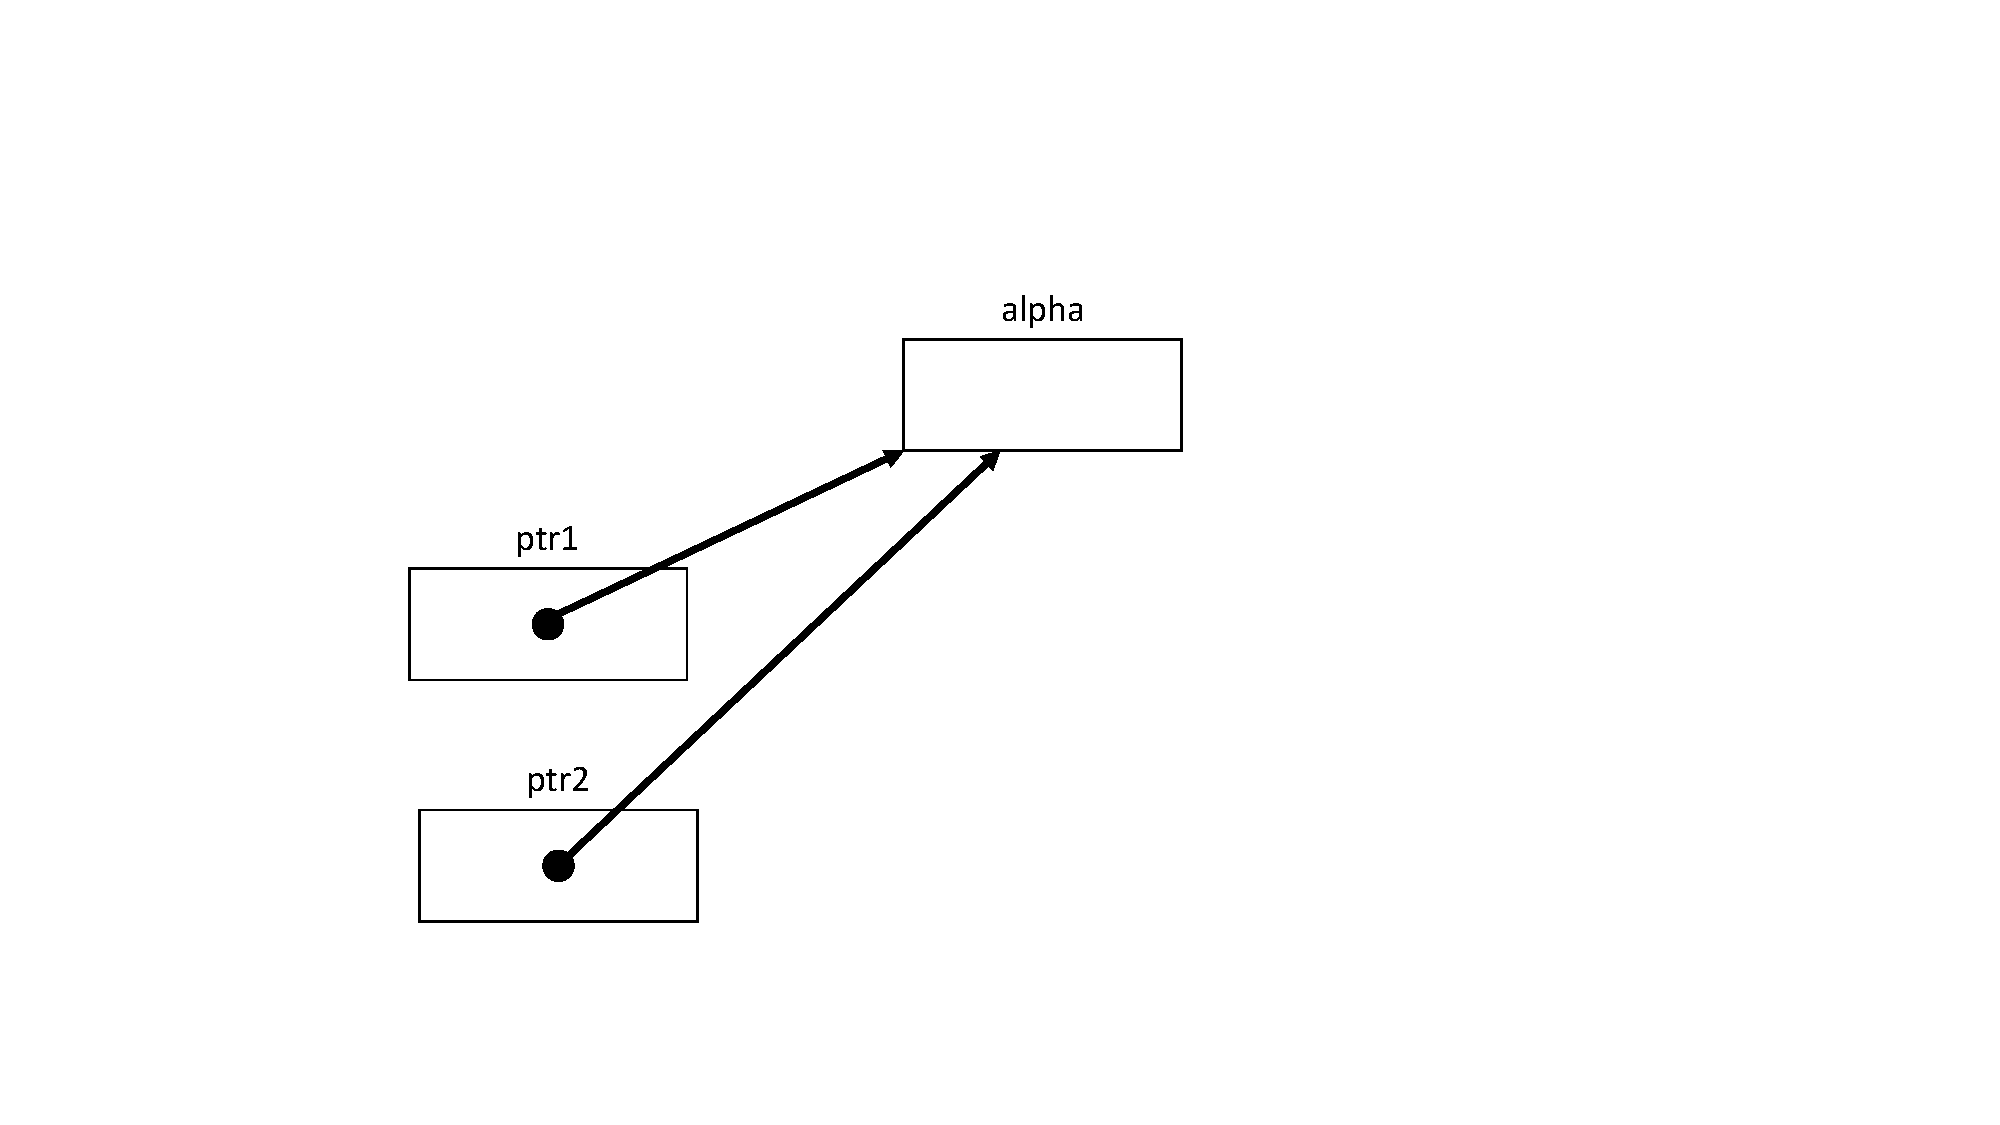
\includegraphics[width=0.4\linewidth]{pointer6.pdf}
\end{figure}
\\ \\ \\

\subsubsection{Der Inhaltsoperator * \textbf{(Dereferenzierung)}\hfill}
\label{sec:unterunterabschnitt}
Ist ptr ein Pointer vom Typ Typname, so liefert der Ausdruck *ptr den Inhalt der Speicherzelle, auf welche ptr zeigt.\\
\\
\noindent
\begin{minipage}{\linewidth}
\begin{lstlisting}
int wert;	// Variable wert vom Typ int wird definiert
int* ptr;	// Pointer ptr auf den Typ int wird definiert
		// ptr zeigt auf eine nicht definierte Adresse
ptr = &wert;	// ptr zeigt nun auf die Variable wert, d.h.
		// ptr enthaelt die Adresse der Variablen wert
*ptr = 23;	// in die Speicherzelle, auf welche ptr zeigt
		// (hier: auf die Variable wert), wird 23 geschrieben.
		// Aequivalent: wert = 23;
\end{lstlisting}
\end{minipage}

\subsubsection{Darstellung in graphischer Pointernotation\hfill}
\label{sec:unterunterabschnitt}
\noindent
\begin{minipage}{\linewidth}
\begin{lstlisting}
int wert;
int* ptr;
ptr = &wert;
\end{lstlisting}
\end{minipage}
\begin{figure}[h]
	\centering
	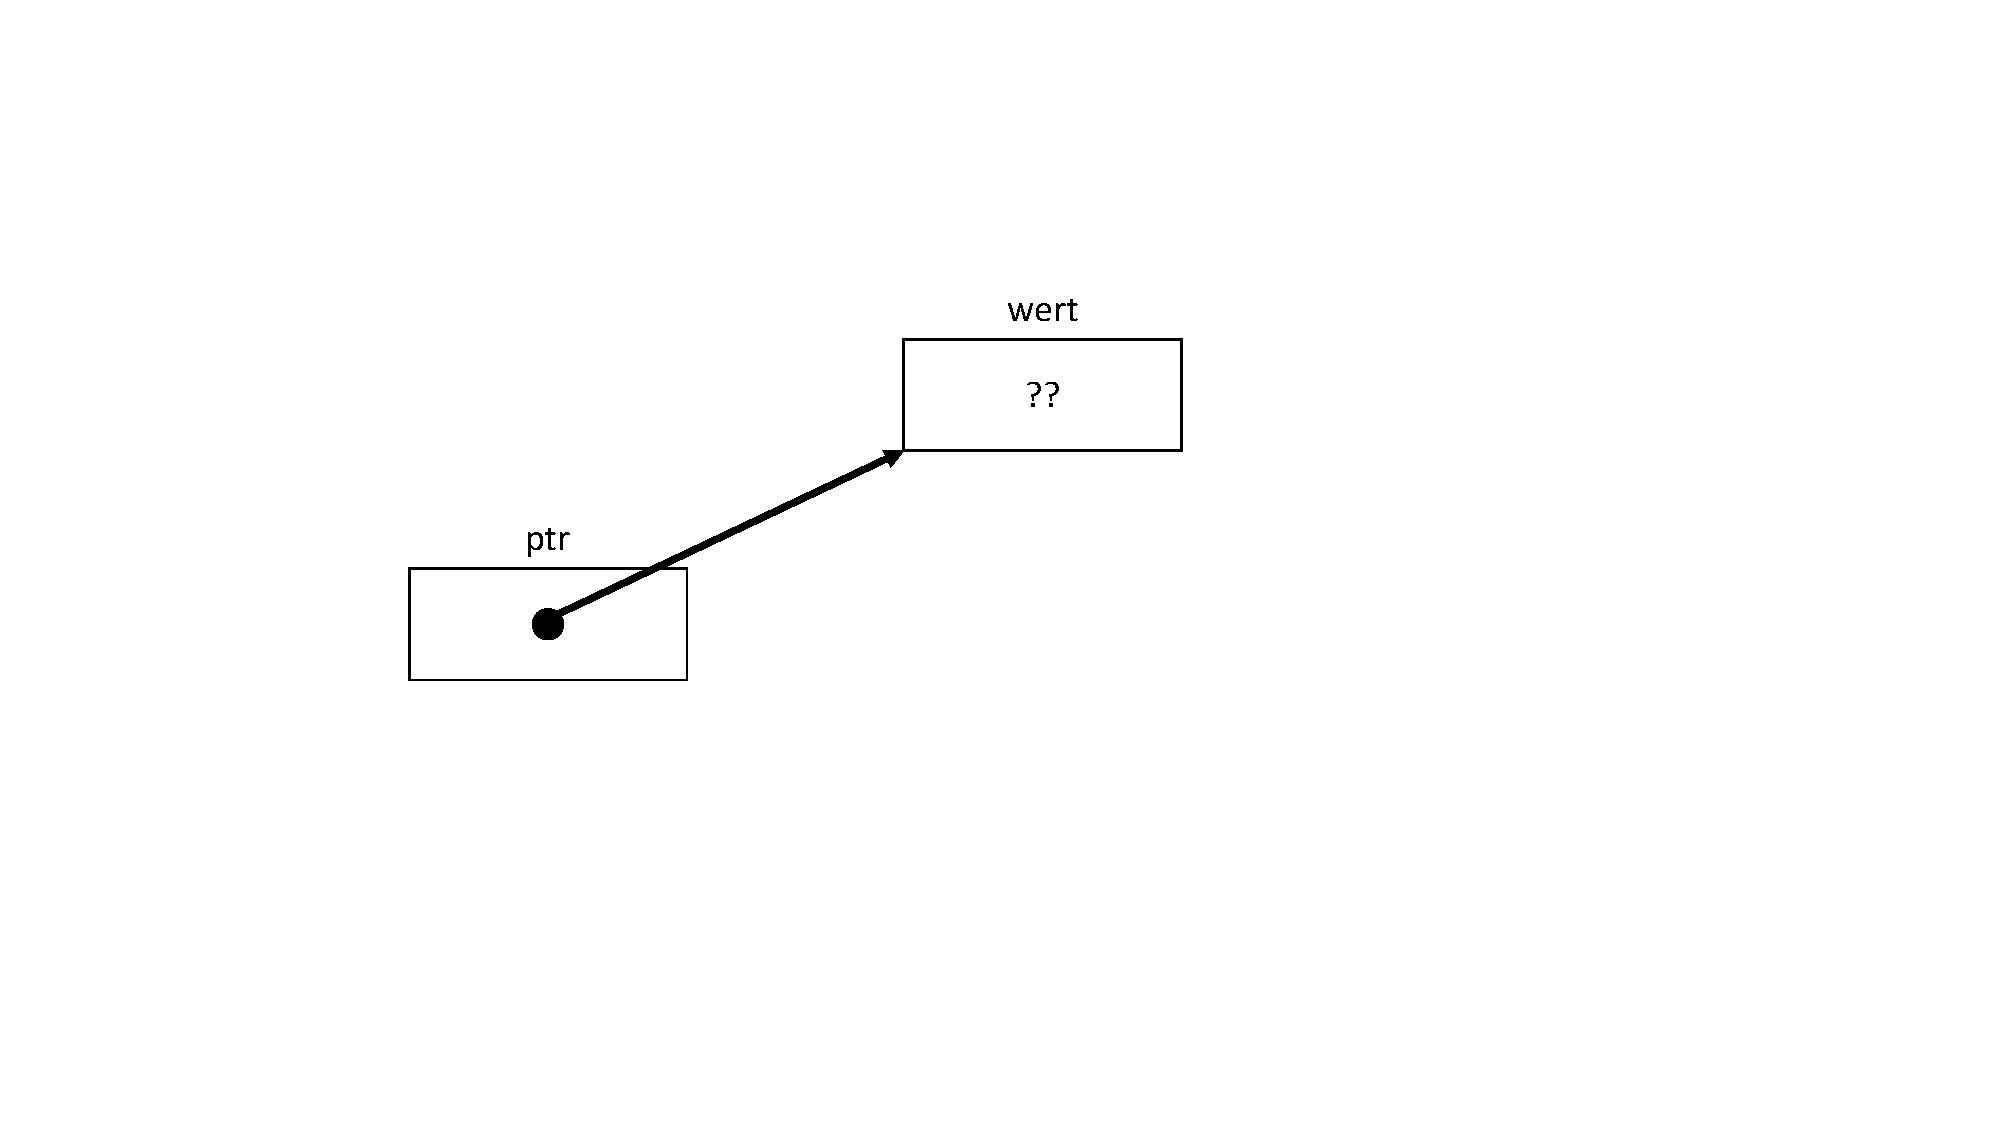
\includegraphics[width=0.4\linewidth]{pointer7.pdf}
\end{figure}
\\ \\ \\
\noindent
\begin{minipage}{\linewidth}
\begin{lstlisting}
*ptr = 23;
\end{lstlisting}
\end{minipage}
\begin{figure}[h]
	\centering
	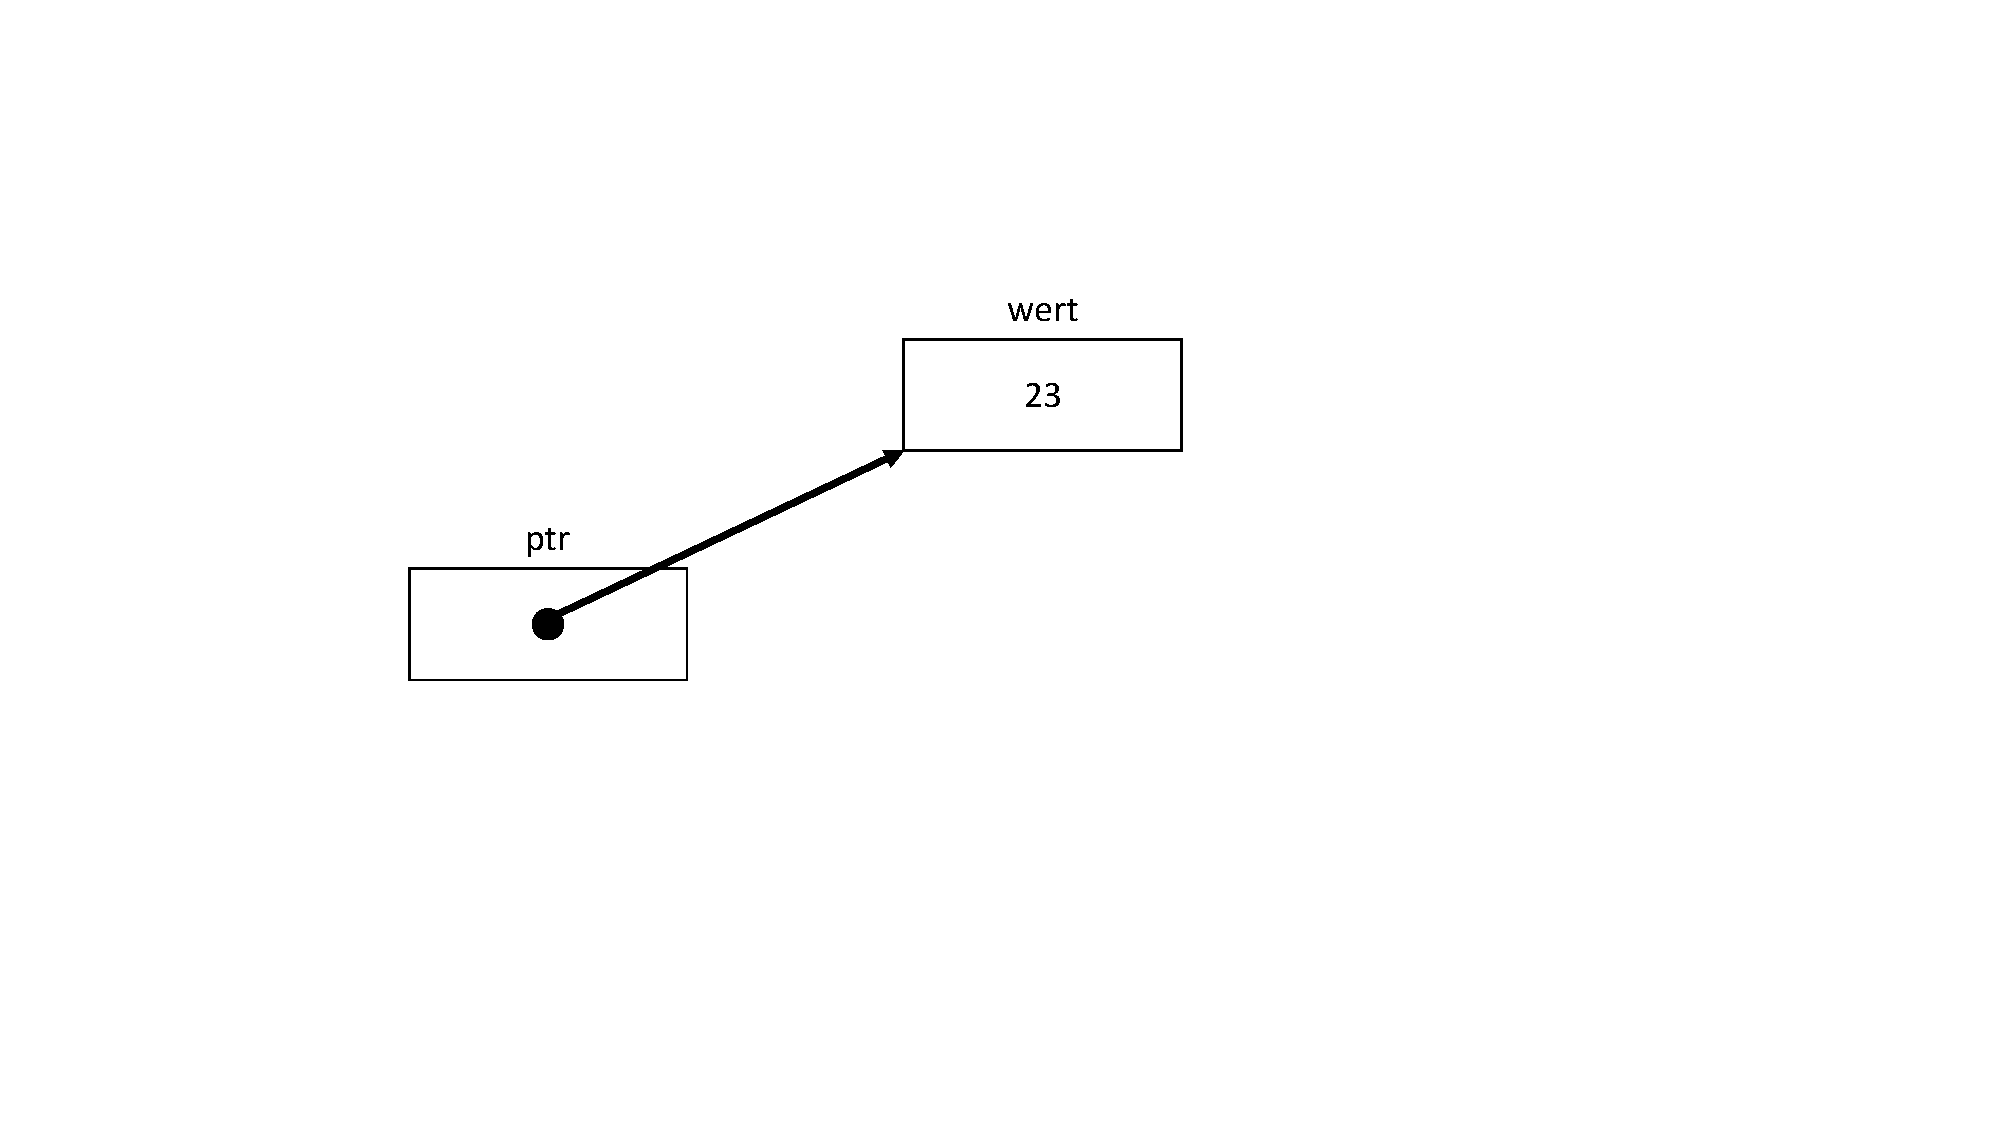
\includegraphics[width=0.4\linewidth]{pointer8.pdf}
\end{figure}
\\ \\ \\

\subsubsection{const bei Pointern: Vorsicht\hfill}
\label{sec:unterunterabschnitt}
\underline{1. Variante: konstanter String}\\
\noindent
\begin{minipage}{\linewidth}
\begin{lstlisting}
char str[] = ''Ein String'';
const char* text = str:
\end{lstlisting}
\end{minipage}
\\
Dies bedeutet nicht, dass der Pointer text konstant ist, sondern dass text auf einen konstanten String zeigt.\\
Von rechts nach links lesen:\\ ''text ist ein Pointer auf eine char-Konstante''\\
\noindent
\begin{minipage}{\linewidth}
\begin{lstlisting}
char ch = text[1];		// erlaubt (==  'i')
text[1] = 's';			*@\color{red}// nicht erlaubt@*
text = ''Ein anderer String'';	// erlaubt
\end{lstlisting}
\end{minipage}
\\ \\ \\ \\
\underline{2. Variante: konstanter Pointer}\\
\noindent
\begin{minipage}{\linewidth}
\begin{lstlisting}
char str[]  = ''Ein String'';
char* const text = strL;
\end{lstlisting}
\end{minipage}
\\
Hier ist nun der Pointer text konstant. Die Position von const ist sehr relevant!\\
Von rechts nach links lesen:\\ ''text ist ein konstanter Pointer auf ein char''\\
\noindent
\begin{minipage}{\linewidth}
\begin{lstlisting}
char ch = test[1];		// erlaubt (== 'i')
text[1] = 's';			// erlaubt
text = ''Ein anderer String'';	*@\color{red}// nicht erlaubt@*
\end{lstlisting}
\end{minipage}
\\ \\ \\ \\
\underline{3. Variante: konstanter Pointer, konstanter String}\\
\noindent
\begin{minipage}{\linewidth}
\begin{lstlisting}
char str[] = ''Ein String'';
const char* const text = str;
\end{lstlisting}
\end{minipage}
\\
Hier ist nun der Pointer text konstant und der Text, wohin er zeigt.\\
Von rechts nach links lesen:\\''text ist ein konstanter Pointer auf eine char-Konstante''\\
\noindent
\begin{minipage}{\linewidth}
\begin{lstlisting}
char ch = text[1];		// erlaubt (== 'i')
text[1] = 's':			*@\color{red}// nicht erlaubt@*
text = ''Ein anderer String'';	*@\color{red}// nicht erlaubt@*
\end{lstlisting}
\end{minipage}
\\ \\ \\ \\
\underline{const bei Pointern in Funktionsköpfen}\\
\noindent
\begin{minipage}{\linewidth}
\begin{lstlisting}
void foo (const int* ptr)
{
	*ptr = 14;		// nicht erlaubt
}
\end{lstlisting}
\end{minipage}
\\
ptr ist ein Pointer auf eine int-Konstante.
\\

\subsubsection{void-Pointer\hfill}
\label{sec:unterunterabschnitt}
\begin{itemize}
	\item void-Pointer sind Objekte, die eine gültige Adresse darstellen
	\item einem void-Pointer kann jeder Pointer zugewiesen werden
	\item \Large{ein void-Pointer kann ohne Typecast nur anderen void-Pointern zugewiesen werden (anders als in C)}\normalsize
	\item ein void-Pointer kann nicht dereferenziert werden
\end{itemize}
\begin{hinweis}
in C++ sollten void-Pointer kaum noch angewendet werden
\end{hinweis}
\underline{void-Pointer: Beispiele}\\
\noindent
\begin{minipage}{\linewidth}
\begin{lstlisting}
int a;
int* pi = &a;
void* pv = pi;			*@\color{green}// ok@*
double* pd = pv			*@\color{red}// Error (in C erlaubt)@*
pd = static_cast<double*>pv;	*@\color{green}// ok@*
\end{lstlisting}
\end{minipage}

\subsubsection{Pointer auf Funktionen\hfill}
\label{sec:unterunterabschnitt}
\begin{itemize}
	\item Jede Funktion befindet sich an einer definierten Adresse im Codespeicher
	\item Diese Adresse kann ebenfalls ermittelt werden
	\item Interessant wäre, dynamisch zur Laufzeit in Abhängigkeit des Programmablaufs eine unterschiedliche Funktion über einen Funktionspointer aufzurufen
\end{itemize}
\begin{hinweis}
In C++ gibt es für viele Situationen bessere Alternativen zu Funktionspointern (Polymorphismus
\end{hinweis}

\subsubsection{Interruptvektortabelle: Tabelle von Funktionspointern\hfill}
\label{sec:unterunterabschnitt}
\centering
\begin{tabularx}{0.25\textwidth}{|X|}
	\hline
	Pointer auf ISR n\\
	\hline
	...\\
	\hline
	...\\
	\hline
	Pointer auf ISR 2\\
	\hline
	Pointer auf ISR 1\\
	\hline
\end{tabularx}
\flushleft
ISR = Interrupt Service Routine

\subsubsection{Umsetzung von Funktionspointern in C/C++\hfill}
\label{sec:unterunterabschnitt}
Der Name der Funktion kann als Adresse auf den ersten Befehl der Funktion verwendet werden (analog Array).

\subsubsection{Beispiel für Funktionspointer}
\label{sec:unterunterabschnitt}
\lstinputlisting{\listings/ftptr.cpp}

% Unterkapitel: Referenzen

\subsection{Referenzen\hfill}
\label{secc:unterabschnitt}

\subsubsection{Was ist eine Referenz?\hfill}
\label{sec:unterunterabschnitt}
\begin{itemize}
	\item Eine Referenz ist ein Alternativname (Alias) für ein Objekt
	\item Referenzen ähneln Pointern, sind aber nicht dasselbe. Bei einem Pointer wird immer eine Adresse ermittelt, d.h. dieses Datenobjekt muss sich im adressierbaren Bereich befinden. Eine Referenz kann aber auch auf ein Register verweisen. Grundsätzlich sind Referenzen effizienter als Pointer.
	\item Syntaktisch sind Referenzen einfacher als Pointer, da ein expliziter Referenzierungs- und Dereferenzierungsoperator entfällt
	\item Referenzen sind für den Programmierer sicherer anzuwenden als Pointer
	\item In gewissen Fällen braucht es Pointer. Wenn nicht, dann sollen Referenzen bevorzugt werden.
\end{itemize}

\subsubsection{Syntax von Referenzen\hfill}
\label{sec:unterunterabschnitt}
\noindent
\begin{minipage}{\linewidth}
\begin{lstlisting}
int x = 24;
int& r1 = x;	// Definition der Referenz r1

x = 55;	// x == 55, r1 == 5 (dasselbe Objekt)
r1 = 7;	// x == 7, r1 == 7 (dasselbe Objekt)
r1++;	// x == 8, r1 == 8 (dasselbe Objekt)
\end{lstlisting}
\end{minipage}
\begin{hinweis}
Referenzen können nach der Definition nicht ''umgehängt'' werden, d.h. eine Referenz kann und muss nur bei der Definition initialisiert werden und kann nicht später auf etwas anders ''zeigen''.
\end{hinweis}

\subsubsection{Einsatz von Referenzen\hfill}
\label{sec:unterunterabschnitt}
\begin{itemize}
	\item In folgenden zwei Fällen einsetzen:
	\begin{itemize}
		\item Bei Parameterübergabe (call by reference) anstatt Pointer (entspricht var-Parameter in der Programmiersprache Pascal)
		\item Bei Referenz-Rückgabetyp anstatt Pointertyp, d.h. als Returntyp
	\end{itemize}
	\item\Large Generell:\\Objekte einer Klasse und Strukturvariablen sollen immer by reference übergeben werden (niemals by value)\normalsize
	\item Sonst: zurückhaltend einsetzen
\end{itemize}

\subsubsection{Pointer und Referenzen auf loiale Variablen\hfill}
\label{sec:unterunterabschnitt}
\begin{achtung}
Sie dürfen niemals einen Pointer oder eine Referenz auf eine lokale Variable oder ein lokales Objekt mittels return zurückgeben
\end{achtung}
Grund:\\Nach Beendigung der Funktion sind die lokalen Variablen ungültig.

% Unterkapitel: Zeiger/Referenzen

\subsection{Zeiger und Referenzen als Parameter und Rückgabewerte\hfill}
\label{sec:unterabschnitt}

\subsubsection{Call by Value vs. Call by Reference\hfill}
\label{sec:unterunterabschnitt}
\begin{itemize}
	\item Parameter, die by value übergeben werden (Wertparameter) werden kopiert, in der Funktion wird mit Kopien gearbeitet.
	\item Bei Referenzparametern (call by reference) wird nur eine Referenz (Alias) des Originals übergeben.
	\item Nur Parameter, welche by reference übergeben werden, könne in der Funktion (bleibend) verändert werden.
\end{itemize}

\subsubsection{3 Beispiele\hfill}
\label{sec:unterunterabschnitt}
\underline{Versuch 1: Call by value}
\noindent
\begin{minipage}{\linewidth}
\begin{lstlisting}
void swap(int a, int b)
{
	int tmp = 1;
	a = b;
	b = tmp;
}

int main()
{
	int x = 4;
	int y = 3;
	swap(x, y);	*@\color{red}// nur Kopien werden vertauscht!\color{black}@*
	return 0;
}
\end{lstlisting}
\end{minipage}
\underline{Versuche 2: Call by reference mit Referenzen}
\noindent
\begin{minipage}{\linewidth}
\begin{lstlisting}
void swap(int& a, int& b)
{
	int tmp = 1;
	a = b;
	b = tmp;
}

int main()
{
	int x = 4;
	int y = 3;
	swap(x, y);	*@\color{green}// OK!\color{black}@*
	return 0;
}
\end{lstlisting}
\end{minipage}
\underline{Versuch 3: Call by reference mit Pointer}
\noindent
\begin{minipage}{\linewidth}
\begin{lstlisting}
void swp(int* a, int* b)
{
	int tmp = *a;
	*a = *b;
	*b = tmp;
}

int main()
{
	int x = 4;
	int y = 3;
	swap(&x, &y);	*@\color{red}// OK, jedoch muehsame Syntax und evtl. ineffizient\color{black}@*
	return 0;
}
\end{lstlisting}
\end{minipage}

\subsubsection{Call by reference: wann einsetzen?\hfill}
\label{sec:unterunterabschnitt}
\#1: wenn Parameter in der Funktion verändert werden sollen\\
\#2: wenn ''grosse'' Parameter übergeben werden sollen (struct, class)\\
zu \#2: wenn verhindert werden soll, dass der Parameter verändert wird, so kann dieser mit const deklariert werden\\
\noindent
\begin{minipage}{\linewidth}
\begin{lstlisting}
int foo(const BigType& b);
\end{lstlisting}
\end{minipage}
\begin{achtung}
Parameterübergabe und Rückgabe von Objekten by value ist ein Hauptgrund für langsame C++-Programme!
\end{achtung}

\subsubsection{Merke\hfill}
\label{sec:unterunterabschnitt}
\begin{achtung}
Variablen einer Struktur und Variablen einer Klasse (Objekte) müssen immer by reference übergeben werden, niemals by value.\\
Read-only Parameter werden zusätzlich mit const spezifiziert.
\end{achtung}
% ENDE

















